\section{Examples}\label{SecExamples}
In this section we illustrate the functioning of the \NAME
library and their interfaces through specific examples, including
discussion of relevant code snippets.
Specifically, we show how the quantum impurity solver in \NAME can be used
to address problems of different nature within the framework of DMFT. 


\subsection{Bethe lattice DMFT (Fortran API)}
The description of the Mott or metal to insulator transition (MIT)
within the Bethe lattice, i.e. Cayley tree with connection
$z\to\infty$ is conventionally considered the test bed of any DMFT
application. Here  we discuss a guided implementation based on the
Fortran API of \NAME of the DMFT solution of the Bethe lattice at
$T=0$. 

We consider a Fermi-Hubbard model:
$$
H = -t \sum_{\langle ij\rangle\s}c^+_{i\s}c_{j\s} + U \sum_i n_{i\up}n_{i\dw}
$$
defined on a Bethe lattice with density of states
$\rho(x)=\frac{1}{2D}\sqrt{D^2-x^2}$, where $D=2t$ is the
half-bandwidth. 

\begin{figure}[t!]
  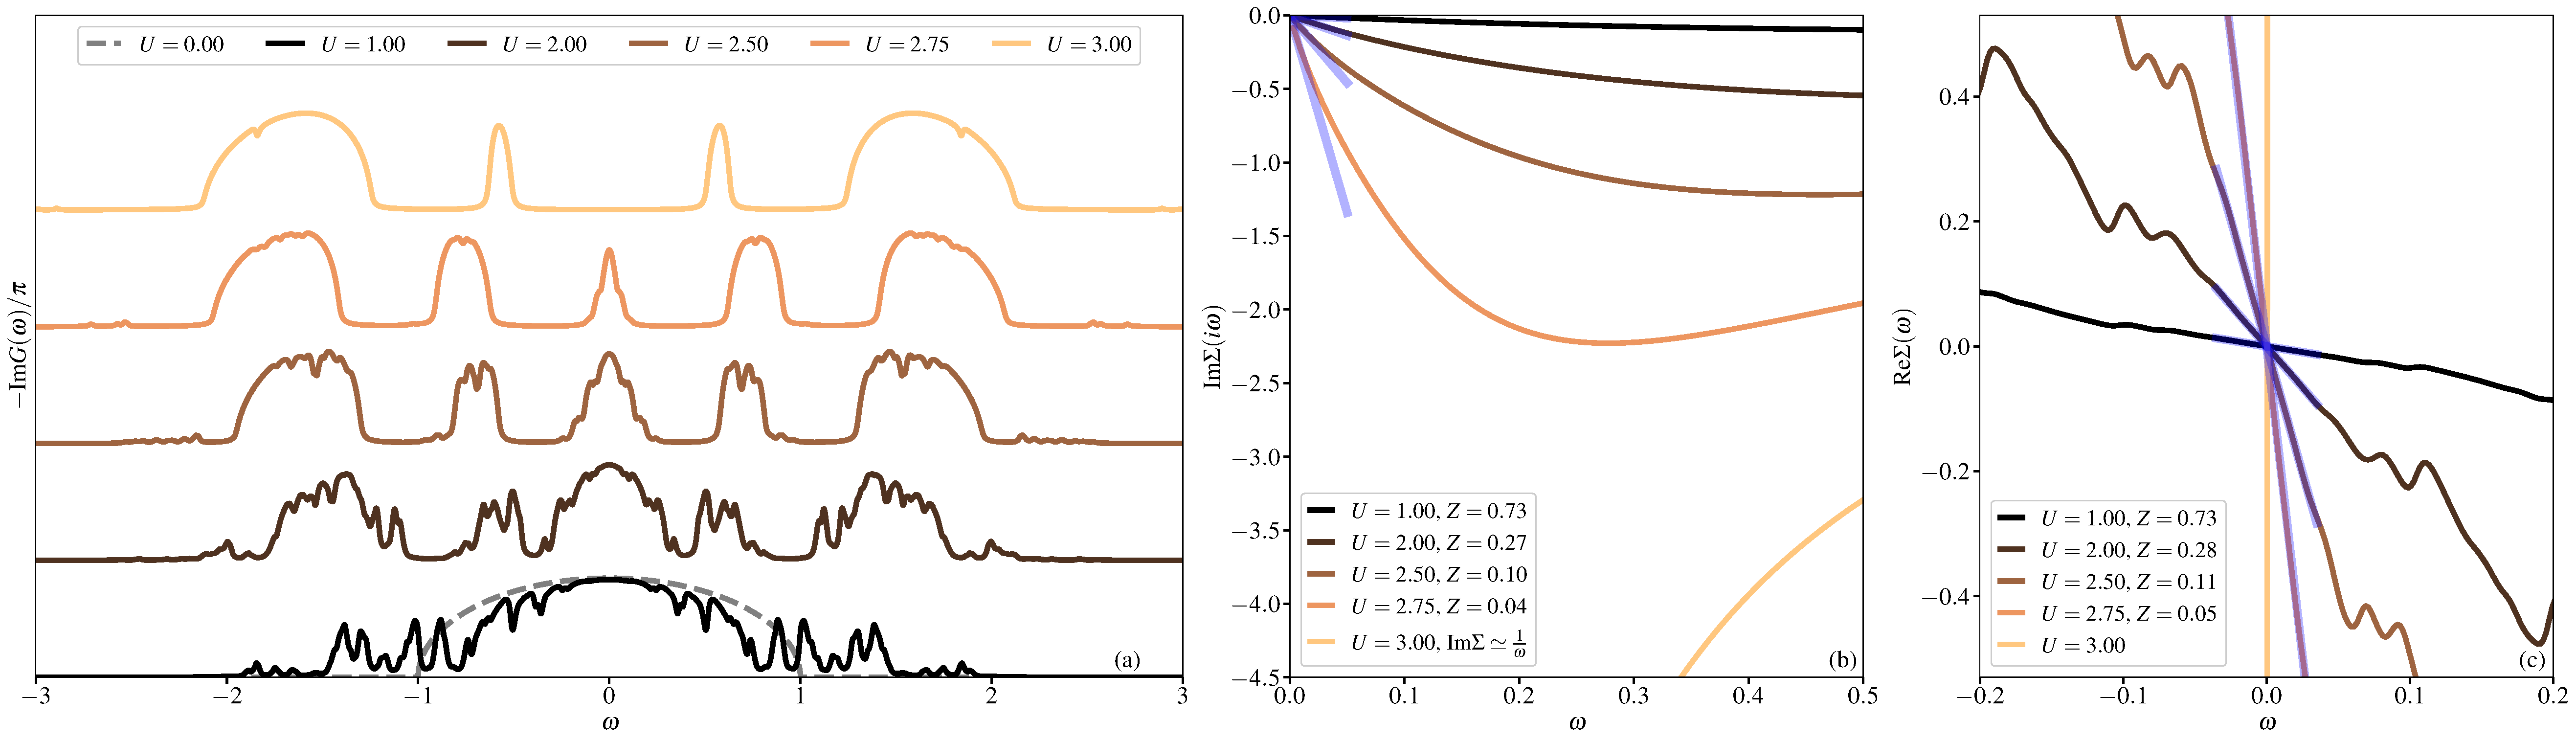
\includegraphics[width=\linewidth]{figures/figBethe.pdf}
    \caption{\label{fig1}%
        \textbf{The Mott transition.}
        }
\end{figure}




\subsection{Attractive Hubbard model (Python API)}
\subsection{Multi-orbital Hubbard (Triqs)}


